\chapter{Overview of the approach}
\label{chap:overview}

The case study concentrates on the connection between the design time and runtime domain, with model based runtime verification using monitors. Our goal is to present the concept of a tool which facilitates the runtime verification design of systems.

\section{Concept of runtime verification with engineering model}

\begin{figure}[h]
	\centering
	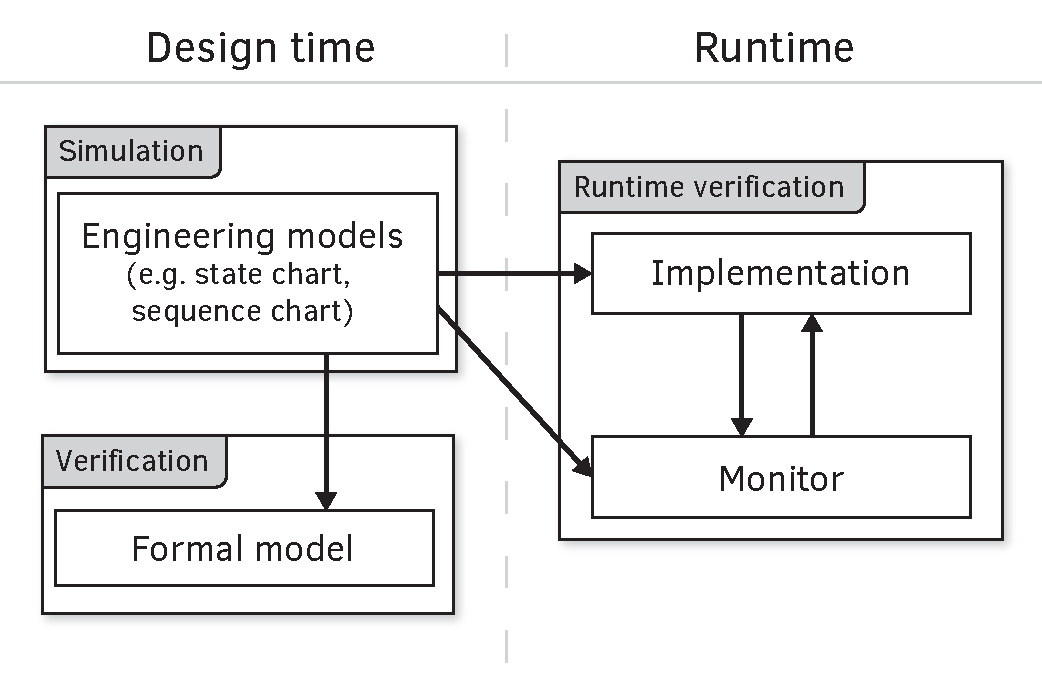
\includegraphics[width=0.6\linewidth]{include/figures/chapter_3/abstract_overview}
	\caption{Connection between runtime and design time elements}
	\label{fig:overview:abstract_overview}
\end{figure}

\cref{fig:overview:abstract_overview} depicts the basic concept. We have three main transformations:
\begin{itemize}
	\item \textbf{Engineering model $\mapsto$ Formal model}: The specified engineering models can be mapped to a formally verifiable transition system.
	\item \textbf{Engineering model $\mapsto$ Implementation}: We can generate components from the engineering models. The generated components then can push state notifications towards the monitor.
	\item \textbf{Engineering model $\mapsto$ Monitor}: The generation of monitoring components is also available (\vref{chap:runtime_verification}) using the engineering models. The monitor is a state machine that is operated by the generated code. If the execution reaches an invalid state, the monitor detects it. After detection the monitor can forward the error detection event to a higher level processor.
\end{itemize}
Some transformation tools exist for these transformations, but there are no tools which integrate all of the above in one framework, allowing multiple formalisms to be used, especially with this level of automation.
\\[1ex]

\noindent Let us consider the following example:

We want to design a system, where we have a logic, described by a formalism (e.g. state chart, sequence chart), and we want to:
\begin{itemize}
	\item Generate the implementation from engineering models.
	\item Implement runtime verification into our implementation, by monitoring it.
	\item Support multiple monitoring systems which can communicate.
\end{itemize}

This example covers the usual need of a distributed, embedded safety logic. We need to formally verify the model, generate code, and monitor it. Our goal is to integrate all these solutions into a generic tool. With a centralized toolchain, a developer can make a system with less effort but with more robustness thanks to the verifiable, and automated steps.
\\[1ex]

\section{Hierarchical runtime verification approach}

We can distinguish three levels, representing the hierarchy of our approach:
\begin{itemize}
	\item \textbf{Local verification with state chart}: With the generated monitor, we could handle the error states locally, e.g. if we detect an error in the generated code, the monitor can react and shut down the system as a precaution.
	\item \textbf{Communication verification with state/sequence chart}: The monitor can verify the communication with the higher level logic, reacting to e.g. loss of communication.
	\item \textbf{Integrating multiple system level monitor}: One way to increase robustness is to connect multiple, independent source of information into the logic. In this way,  
\end{itemize}

If we specify a high level specification to our overall system, which can have many monitored, communicating components, we can build a high level logic on top of these components offering another level of monitoring, and robustness.

\begin{figure}[h]
	\centering
	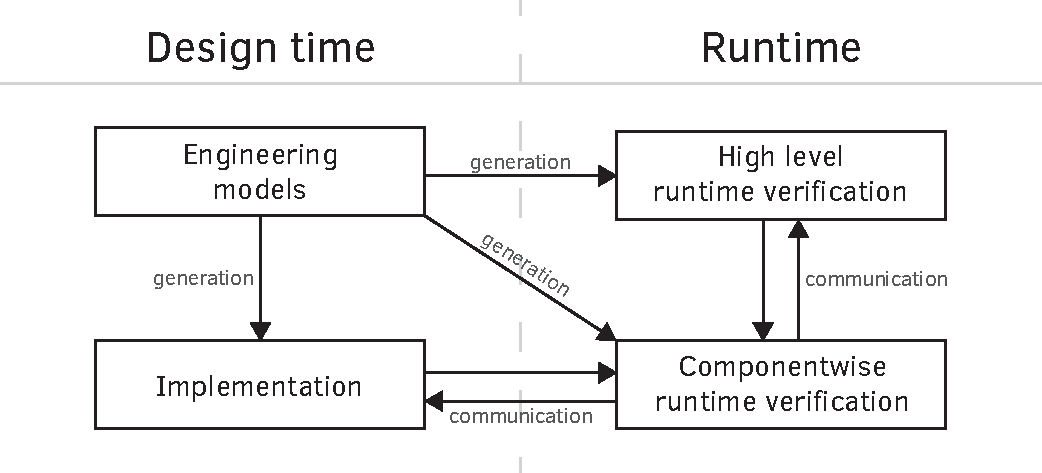
\includegraphics[width=0.8\linewidth]{include/figures/chapter_3/abstract_diagram}
	\caption{Conceptual draw of a hierarchical system element relations with our method}
	\label{fig:overview:abstract_diagram}
\end{figure}

As \cref{fig:overview:abstract_diagram} shows, a hierarchical solution can be made by just defining the correct engineering model, and the high level logic can automatically intercept the error state messages.

The high level logic can range from simple reaction logic to a complex system, like the complex event processing solution (\vref{chap:cep}).
